\chapter{Conditional Probability}
\label{chapter:ConditionalProbability}

Conditional probability provides a way to compute the likelihood of an event based on \emph{partial information}.
This is a powerful concept that is used extensively throughout engineering with applications to decision making, networks, communications and many other fields.


\section{Conditioning on Events}

We begin our description of conditional probability with illustrative examples.
The intuition gained through this exercise is then generalized by introducing a formal definition for this important concept.

\begin{example}
The rolling of a fair die is an experiment with six equally likely outcomes.
As such, the probability of obtaining any of the outcomes is $1/6$.
However, if we are told that the upper face features an odd number, then only three possibilities remain, namely $\{1, 3, 5 \}$.
\begin{figure}[htb!]
\begin{center}
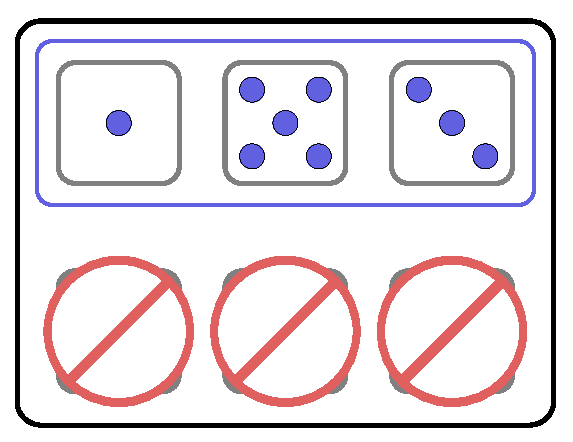
\includegraphics[height=3.675cm]{Figures/3Chapter/condevent}
\caption{Partial information about the outcome of an experiment may change the likelihood of events.
The resulting values are known as conditional probabilities.}
\label{figure:CondEvent}
\end{center}
\end{figure}
These three outcomes had equal probabilities before the additional information was revealed.
It then seems natural to assume that they remain equally likely afterwards.
In particular, it is reasonable to assign a probability of $1/3$ to each of the three outcomes that remain possible candidates after receiving the side information.
We can express the probability of getting a three given that the outcome is an odd number as
\begin{equation*}
\frac{\Pr (3 \cap \{ 1, 3, 5 \})}{\Pr (\{ 1, 3, 5 \} ) }
= \frac{\Pr(3)}{\Pr (\{1,3,5\})} = \frac{1}{3} .
\end{equation*}
\end{example}

\begin{example}
Let $A$ and $B$ be events associated with a random experiment, and assume that $\Pr(B)>0$.
To gain additional insight into conditional probability, we consider the scenario where this experiment is repeated $N$ times.
Let $N_{AB}$ be the number of trials for which $A \cap B$ occurs, $N_{A\overline{B}}$ be the number of times where only $A$ occurs,  $N_{\overline{A}B}$ be the number of times where only $B$ occurs, and  $N_{\overline{A}\overline{B}}$ be the number of trials for which neither takes place.
From these definitions, we gather that $A$ is observed exactly $N_A = N_{AB} + N_{A\overline{B}}$ times, and $B$ is seen $N_B = N_{AB} + N_{\overline{A}B}$ times.

The frequentist view of probability is based on the fact that, as $N$ becomes large, one can approximate the probability of an event by taking the ratio of the number of times this event occurs over the total number of trials.
For instance, we can write
\begin{xalignat*}{2}
\Pr (A\cap B) & \approx \frac{N_{AB}}{N} &
\Pr (B) & \approx \frac{N_{B}}{N}.
\end{xalignat*}
Likewise, the conditional probability of $A$ given knowledge that the outcome lies in $B$ can be computed using
\begin{equation} \label{equation:FrequentistApproximation}
\Pr (A | B) \approx \frac{N_{AB}}{N_B}
= \frac{N_{AB} / N}{N_B / N} \approx \frac{\Pr (A \cap B)}{\Pr (B)}.
\end{equation}
As $N$ approaches infinity, these approximations become exact and \eqref{equation:FrequentistApproximation} unveils the formula for conditional probability.
\end{example}

Having considered intuitive arguments, we turn to the mathematical definition of conditional probability.
Let $B$ be an event such that $\Pr (B) > 0$.
A conditional probability law assigns to every event $A$ a number $\Pr (A|B)$, termed the \emph{conditional probability of $A$ given $B$}, such that \index{Conditional probability}
\begin{equation} \label{equation:ConditionalProbability}
\Pr (A | B) = \frac{\Pr (A \cap B)}{\Pr (B)}.
\end{equation}
We can show that the collection of conditional probabilities $\{ \Pr (A | B) \}$ specifies a valid probability law, as defined in Section~\ref{section:ProbabilityLaws}.
For every event $A$, we have
\begin{equation*}
\Pr (A|B) = \frac{\Pr (A \cap B)}{\Pr (B)} \geq 0
\end{equation*}
and, hence, $\Pr (A|B)$ is nonnegative.
The probability of the entire sample space $\Omega$ is equal to
\begin{equation*}
\Pr (\Omega | B) = \frac{\Pr (\Omega \cap B)}{\Pr (B)}
= \frac{\Pr (B)}{\Pr (B)} = 1 .
\end{equation*}
If $A_1, A_2, \ldots$ is a sequence of disjoint events, then
\begin{equation*}
A_1 \cap B, A_2 \cap B, \ldots
\end{equation*}
is also a sequence of disjoint events and
\begin{equation*}
\begin{split}
\Pr \left( \bigcup_{k=1}^{\infty} A_k \Big| B \right)
&= \frac{\Pr \left( \left( \bigcup_{k=1}^{\infty} A_k \right) \cap B \right)}{\Pr (B)}
= \frac{\Pr \left( \bigcup_{k=1}^{\infty} (A_k \cap B ) \right)}{\Pr (B)} \\
&= \sum_{k = 1}^{\infty} \frac{ \Pr (A_k \cap B ) }{\Pr (B)}
= \sum_{k = 1}^{\infty} \Pr (A_k | B) ,
\end{split}
\end{equation*}
where the third equality follows from the third axiom of probability applied to the set $\bigcup_{k=1}^{\infty} (A_k \cap B )$.
Thus, the conditional probability law defined by \eqref{equation:ConditionalProbability} satisfies the three axioms of probability.

\begin{example}
A fair coin is tossed repetitively until heads is observed.
In Example~\ref{example:CoinTossSequence}, we found that the probability of observing heads for the first time on trial $k$ is $2^{-k}$.
We now wish to compute the probability that heads occurred for the first time on the second trial given that it took an even number of tosses to observe heads.
In this example, $A = \{ 2 \}$ and $B$ is the set of even numbers.
The probability that the outcome is two, given that the number of tosses is even, is equal to
\begin{equation*}
\Pr ( 2 | B )
= \frac{\Pr ( 2 \cap B )}{\Pr (B)}
= \frac{\Pr (2)}{\Pr (B)}
= \frac{1/4}{1/3}
= \frac{3}{4} .
\end{equation*}
In the above computation, we have used the fact that the probability of flipping the coin an even number of times is equal to $1/3$.
This fact was established in Example~\ref{example:CoinTossSequence}.
\end{example}

The definition of conditional probability can be employed to compute the probability of several events occurring simultaneously.
Let $A_1, A_2, \ldots, A_n$ be a collection of events.
The probability of events $A_1$ through $A_n$ taking place at the same time is given by
\begin{equation} \label{equation:SimultaneousEvents}
\Pr \left( \bigcap_{k=1}^n A_k \right)
= \Pr (A_1) \Pr (A_2 | A_1) \Pr (A_3 | A_1 \cap A_2)
\cdots \Pr \left( A_n \bigg| \bigcap_{k=1}^{n-1} A_k \right) .
\end{equation}
This formula is known as the \emph{chain rule of probability}, and it can be verified by expanding each of the conditional probabilities using \eqref{equation:ConditionalProbability},
\begin{equation*}
\Pr \left( \bigcap_{k=1}^n A_k \right)
= \Pr (A_1) \frac{\Pr (A_1 \cap A_2)}{\Pr (A_1)}
\frac{\Pr (A_1 \cap A_2 \cap A_3)}{\Pr (A_1 \cap A_2)}
\cdots \frac{\Pr \left( \bigcap_{k=1}^{n} A_k \right)}
{\Pr \left( \bigcap_{k=1}^{n-1} A_k \right)} .
\end{equation*}
This latter expression implicitly assumes that $\Pr \left( \bigcap_{k=1}^{n-1} A_k \right) \neq 0$.

\begin{example}
An urn contains eight blue balls and four green balls.
Three balls are drawn from this urn without replacement.
We wish to compute the probability that all three balls are blue.
The probability of drawing a blue ball the first time is equal to $8/12$.
The probability of drawing a blue ball the second time given that the first ball is blue is $7/11$.
Finally, the probability of drawing a blue ball the third time given that the first two balls are blue is $6/10$.
Using \eqref{equation:SimultaneousEvents}, we can compute the probability of drawing three blue balls as
\begin{equation*}
\Pr (bbb)
= \frac{8}{12} \frac{7}{11} \frac{6}{10}
= \frac{14}{55} .
\end{equation*}

\begin{figure}[htb!]
\begin{center}
% FIGURE GROUP = BALLS
\begin{footnotesize}
\begin{tikzpicture}
\shade[draw=black, ball color=blue, circular drop shadow] (0.9,1.732) circle (4mm);
\shade[fill=white, fill opacity=0.3] (0.9,1.732) circle (4mm) node[fill opacity=1]{2};

\shade[draw=black, ball color=red, circular drop shadow] (0.45,0.866) circle (4mm);
\shade[fill=white, fill opacity=0.3] (0.45,0.866) circle (4mm) node[fill opacity=1]{1};
\shade[draw=black, ball color=red, circular drop shadow] (1.35,0.866) circle (4mm);
\shade[fill=white, fill opacity=0.3] (1.35,0.866) circle (4mm) node[fill opacity=1]{1};
\shade[draw=black, ball color=blue, circular drop shadow] (2.25,0.866) circle (4mm);
\shade[fill=white, fill opacity=0.3] (2.25,0.866) circle (4mm) node[fill opacity=1]{2};
\shade[draw=black, ball color=red, circular drop shadow] (3.15,0.866) circle (4mm);
\shade[fill=white, fill opacity=0.3] (3.15,0.866) circle (4mm) node[fill opacity=1]{1};

\shade[draw=black, ball color=red, circular drop shadow] (0,0) circle (4mm);
\shade[fill=white, fill opacity=0.3] (0,0) circle (4mm) node[fill opacity=1]{1};
\shade[draw=black, ball color=blue, circular drop shadow] (0.9,0) circle (4mm);
\shade[fill=white, fill opacity=0.3] (0.9,0) circle (4mm) node[fill opacity=1]{2};
\shade[draw=black, ball color=red, circular drop shadow] (1.8,0) circle (4mm);
\shade[fill=white, fill opacity=0.3] (1.8,0) circle (4mm) node[fill opacity=1]{1};
\shade[draw=black, ball color=red, circular drop shadow] (2.7,0) circle (4mm);
\shade[fill=white, fill opacity=0.3] (2.7,0) circle (4mm) node[fill opacity=1]{1};
\shade[draw=black, ball color=blue, circular drop shadow] (3.6,0) circle (4mm);
\shade[fill=white, fill opacity=0.3] (3.6,0) circle (4mm) node[fill opacity=1]{2};

\draw[very thick, ->, >=stealth'] (4.6,0.866) -- (5.6,0.866);

\shade[draw=black, ball color=red, circular drop shadow] (6.6,0.866) circle (4mm);
\shade[fill=white, fill opacity=0.3] (6.6,0.866) circle (4mm) node[fill opacity=1]{1};
\shade[draw=black, ball color=red, circular drop shadow] (7.6,0.866) circle (4mm);
\shade[fill=white, fill opacity=0.3] (7.6,0.866) circle (4mm) node[fill opacity=1]{1};
\draw[draw=black] (8.6,0.866) circle (4mm);

\shade[draw=black, ball color=blue, circular drop shadow] (0.9,4.732) circle (4mm);
\shade[fill=white, fill opacity=0.3] (0.9,4.732) circle (4mm) node[fill opacity=1]{2};
\shade[draw=black, ball color=red, circular drop shadow] (1.8,4.732) circle (4mm);
\shade[fill=white, fill opacity=0.3] (1.8,4.732) circle (4mm) node[fill opacity=1]{1};

\shade[draw=black, ball color=red, circular drop shadow] (0.45,3.866) circle (4mm);
\shade[fill=white, fill opacity=0.3] (0.45,3.866) circle (4mm) node[fill opacity=1]{1};
\shade[draw=black, ball color=red, circular drop shadow] (1.35,3.866) circle (4mm);
\shade[fill=white, fill opacity=0.3] (1.35,3.866) circle (4mm) node[fill opacity=1]{1};
\shade[draw=black, ball color=blue, circular drop shadow] (2.25,3.866) circle (4mm);
\shade[fill=white, fill opacity=0.3] (2.25,3.866) circle (4mm) node[fill opacity=1]{2};
\shade[draw=black, ball color=red, circular drop shadow] (3.15,3.866) circle (4mm);
\shade[fill=white, fill opacity=0.3] (3.15,3.866) circle (4mm) node[fill opacity=1]{1};

\shade[draw=black, ball color=red, circular drop shadow] (0,3) circle (4mm);
\shade[fill=white, fill opacity=0.3] (0,3) circle (4mm) node[fill opacity=1]{1};
\shade[draw=black, ball color=blue, circular drop shadow] (0.9,3) circle (4mm);
\shade[fill=white, fill opacity=0.3] (0.9,3) circle (4mm) node[fill opacity=1]{2};
\shade[draw=black, ball color=red, circular drop shadow] (1.8,3) circle (4mm);
\shade[fill=white, fill opacity=0.3] (1.8,3) circle (4mm) node[fill opacity=1]{1};
\shade[draw=black, ball color=red, circular drop shadow] (2.7,3) circle (4mm);
\shade[fill=white, fill opacity=0.3] (2.7,3) circle (4mm) node[fill opacity=1]{1};
\shade[draw=black, ball color=blue, circular drop shadow] (3.6,3) circle (4mm);
\shade[fill=white, fill opacity=0.3] (3.6,3) circle (4mm) node[fill opacity=1]{2};

\draw[very thick, ->, >=stealth'] (4.6,3.866) -- (5.6,3.866);

\shade[draw=black, ball color=red, circular drop shadow] (6.6,3.866) circle (4mm);
\shade[fill=white, fill opacity=0.3] (6.6,3.866) circle (4mm) node[fill opacity=1]{1};
\draw[draw=black] (7.6,3.866) circle (4mm);
\draw[draw=black] (8.6,3.866) circle (4mm);

\shade[draw=black, ball color=blue, circular drop shadow] (0.9,7.732) circle (4mm);
\shade[fill=white, fill opacity=0.3] (0.9,7.732) circle (4mm) node[fill opacity=1]{2};
\shade[draw=black, ball color=red, circular drop shadow] (1.8,7.732) circle (4mm);
\shade[fill=white, fill opacity=0.3] (1.8,7.732) circle (4mm) node[fill opacity=1]{1};
\shade[draw=black, ball color=red, circular drop shadow] (2.7,7.732) circle (4mm);
\shade[fill=white, fill opacity=0.3] (2.7,7.732) circle (4mm) node[fill opacity=1]{1};

\shade[draw=black, ball color=red, circular drop shadow] (0.45,6.866) circle (4mm);
\shade[fill=white, fill opacity=0.3] (0.45,6.866) circle (4mm) node[fill opacity=1]{1};
\shade[draw=black, ball color=red, circular drop shadow] (1.35,6.866) circle (4mm);
\shade[fill=white, fill opacity=0.3] (1.35,6.866) circle (4mm) node[fill opacity=1]{1};
\shade[draw=black, ball color=blue, circular drop shadow] (2.25,6.866) circle (4mm);
\shade[fill=white, fill opacity=0.3] (2.25,6.866) circle (4mm) node[fill opacity=1]{2};
\shade[draw=black, ball color=red, circular drop shadow] (3.15,6.866) circle (4mm);
\shade[fill=white, fill opacity=0.3] (3.15,6.866) circle (4mm) node[fill opacity=1]{1};

\shade[draw=black, ball color=red, circular drop shadow] (0,6) circle (4mm);
\shade[fill=white, fill opacity=0.3] (0,6) circle (4mm) node[fill opacity=1]{1};
\shade[draw=black, ball color=blue, circular drop shadow] (0.9,6) circle (4mm);
\shade[fill=white, fill opacity=0.3] (0.9,6) circle (4mm) node[fill opacity=1]{2};
\shade[draw=black, ball color=red, circular drop shadow] (1.8,6) circle (4mm);
\shade[fill=white, fill opacity=0.3] (1.8,6) circle (4mm) node[fill opacity=1]{1};
\shade[draw=black, ball color=red, circular drop shadow] (2.7,6) circle (4mm);
\shade[fill=white, fill opacity=0.3] (2.7,6) circle (4mm) node[fill opacity=1]{1};
\shade[draw=black, ball color=blue, circular drop shadow] (3.6,6) circle (4mm);
\shade[fill=white, fill opacity=0.3] (3.6,6) circle (4mm) node[fill opacity=1]{2};

\draw[very thick, ->, >=stealth'] (4.6,6.866) -- (5.6,6.866);

\draw[draw=black] (6.6,6.866) circle (4mm);
\draw[draw=black] (7.6,6.866) circle (4mm);
\draw[draw=black] (8.6,6.866) circle (4mm);
\end{tikzpicture}
\end{footnotesize}
\caption{Conditional probabilities can be employed to calculate the probability of multiple events occurring at the same time.}
\label{figure:Balls}
\end{center}
\end{figure}
\end{example}


\section{The Total Probability Theorem}

The probability of events $A$ and $B$ occurring at the same time can be calculated as a special case of \eqref{equation:SimultaneousEvents}.
For two events, this computational formula simplifies to
\begin{equation} \label{equation:ProbabilityIntersection}
\Pr (A \cap B) = \Pr (A|B) \Pr (B) .
\end{equation}
We can also obtain this equation directly from the definition of conditional probability.
This property is a key observation that plays a central role in establishing two important results, the \emph{total probability theorem} and \emph{Bayes' rule}.
To formulate these two theorems, we need to revisit the notion of a partition.
A collection of events $A_1, A_2, \ldots, A_n$ is said to be a \emph{partition} of the sample space $\Omega$ if these events are disjoint and their union is the entire sample space, \index{Partition}
\begin{equation*}
\bigcup_{k=1}^n A_k = \Omega .
\end{equation*}
Visually, a partition divides an entire set into disjoint subsets, as exemplified in Figure~\ref{figure:SetPartitiion2}.

\begin{figure}[htb]
\begin{center}
\begin{tikzpicture}
\begin{scope}
    \clip (-2cm,-2cm) rectangle (-0.5cm,2cm);
    \draw[thick,fill=red!20] (0,0) circle (1.5cm);
\end{scope}
\begin{scope}
    \clip (-0.5cm,-2cm) rectangle (0.5cm,2cm);
    \draw[thick,fill=green!20] (0,0) circle (1.5cm);
\end{scope}
\begin{scope}
    \clip (0.5cm,-2cm) rectangle (2cm,2cm);
    \draw[thick,fill=blue!20] (0,0) circle (1.5cm);
\end{scope}
\begin{scope}
    \clip (0,0) circle (1.5cm);
    \draw[thick] (-0.5cm,-2cm) rectangle (0.5cm,2cm);
\end{scope}
\coordinate [label=center:{$A_1$}] (A1b) at (-1cm,0);
\coordinate [label=center:{$A_2$}] (A2b) at (0cm,0);
\coordinate [label=center:{$A_3$}] (A3b) at (1cm,0);

\begin{scope}
    \clip (3.5cm,-2cm) rectangle (5cm,2cm);
    \draw[thick,fill=red!20] (5.5cm,0) circle (1.5cm);
\end{scope}
\begin{scope}
    \clip (5.5cm,0) circle (1.5cm);
    \draw[thick] (3.5cm,-2cm) rectangle (5cm,2cm);
\end{scope}
\begin{scope}
    \clip (5.5cm,-2cm) rectangle (6.5cm,2cm);
    \draw[thick,fill=green!20] (6cm,0) circle (1.5cm);
\end{scope}
\begin{scope}
    \clip (6cm,0) circle (1.5cm);
    \draw[thick] (5.5cm,-2cm) rectangle (6.5cm,2cm);
\end{scope}
\begin{scope}
    \clip (7cm,-2cm) rectangle (8.5cm,2cm);
    \draw[thick,fill=blue!20] (6.5cm,0) circle (1.5cm);
\end{scope}
\begin{scope}
    \clip (6.5cm,0) circle (1.5cm);
    \draw[thick] (7cm,-2cm) rectangle (8.5cm,2cm);
\end{scope}
\coordinate [label=center:{$A_1$}] (A1a) at (4.5cm,0);
\coordinate [label=center:{$A_2$}] (A2a) at (6cm,0);
\coordinate [label=center:{$A_3$}] (A3a) at (7.5cm,0);

\draw[->,thick,>=stealth'] (2.25cm,0) to (3.25cm,0);
\end{tikzpicture}
\caption{A partition of $\Omega$ can be formed by selecting a collection of subsets that are disjoint and whose union is $\Omega$.}
\label{figure:SetPartitiion2}
\end{center}
\end{figure}

\begin{theorem}[Total Probability Theorem] \label{theorem:TotalProbability} \index{Total probability theorem}
Let $A_1, A_2, \ldots, A_n$ be a collection of events that forms a partition of the sample space $\Omega$.
Suppose that $\Pr (A_k) > 0$ for all $k$.
Then, for any event $B$, we can write
\begin{equation*}
\begin{split}
\Pr (B) &= \Pr (A_1 \cap B) + \Pr (A_2 \cap B) + \cdots + \Pr (A_n \cap B) \\
&= \Pr (A_1) \Pr (B | A_1) + \Pr (A_2) \Pr (B | A_2) + \cdots + \Pr (A_n) \Pr (B | A_n ) .
\end{split}
\end{equation*}
\end{theorem}
\begin{proof}
The collection of events $A_1, A_2, \ldots, A_n$ forms a partition of the sample space $\Omega$.
We can therefore write
\begin{equation*}
B = B \cap \Omega = B \cap \left( \bigcup_{k=1}^n A_k \right) .
\end{equation*}
Since $A_1, A_2, \ldots, A_n$ are disjoint sets, the events $A_1 \cap B, A_2 \cap B, \ldots, A_n \cap B$ are also disjoint.
Combining these two facts, we get
\begin{equation*}
\begin{split}
\Pr (B)
&= \Pr \left( B \cap \left( \bigcup_{k=1}^n A_k \right) \right)
= \Pr \left( \bigcup_{k=1}^n (B \cap A_k) \right) \\
&= \sum_{k=1}^n \Pr \left( B \cap A_k \right)
= \sum_{k=1}^n \Pr (A_k) \Pr \left( B |A_k \right) ,
\end{split}
\end{equation*}
where the fourth equality follows from the third axiom of probability.
\end{proof}

\begin{figure}[htb]
\begin{center}
\begin{tikzpicture}
\draw[thick,fill=black!10] (0,0) circle (1.5cm);
\draw[thick,fill=yellow!20] (-1cm,-1cm) rectangle (1cm,1cm);
\coordinate [label=center:{$B$}] (B) at (0,0);

\begin{scope}
    \clip (3.5cm,-2cm) rectangle (5cm,2cm);
    \draw[thick,fill=black!10] (5.5cm,0) circle (1.5cm);
    \draw[thick,fill=red!20] (4.5cm,-1cm) rectangle (5.5cm,1cm);
\end{scope}
\begin{scope}
    \clip (5.5cm,0) circle (1.5cm);
    \draw[thick] (3.5cm,-2cm) rectangle (5cm,2cm);
\end{scope}
\begin{scope}
    \clip (5.5cm,-2cm) rectangle (6.5cm,2cm);
    \draw[thick,fill=black!10] (6cm,0) circle (1.5cm);
    \draw[thick,fill=green!20] (5cm,-1cm) rectangle (7cm,1cm);
\end{scope}
\begin{scope}
    \clip (6cm,0) circle (1.5cm);
    \draw[thick] (5.5cm,-2cm) rectangle (6.5cm,2cm);
\end{scope}
\begin{scope}
    \clip (7cm,-2cm) rectangle (8.5cm,2cm);
    \draw[thick,fill=black!10] (6.5cm,0) circle (1.5cm);
    \draw[thick,fill=blue!20] (5.5cm,-1cm) rectangle (7.5cm,1cm);
\end{scope}
\begin{scope}
    \clip (6.5cm,0) circle (1.5cm);
    \draw[thick] (7cm,-2cm) rectangle (8.5cm,2cm);
\end{scope}
\coordinate [label=center:{$B \cap A_1$}] (BA1) at (4cm,-1.75cm);
\draw[->,thick,>=stealth'] (4.15cm,-1.5cm) to (4.75cm,-0.5cm);
\coordinate [label=center:{$B \cap A_2$}] (BA2) at (6cm,-2cm);
\draw[->,thick,>=stealth'] (6cm,-1.75cm) to (6cm,-0.5cm);
\coordinate [label=center:{$B \cap A_3$}] (BA3) at (8cm,-1.75cm);
\draw[->,thick,>=stealth'] (7.85cm,-1.5cm) to (7.25cm,-0.5cm);

\draw[->,thick,>=stealth'] (2.25cm,0) to (3.25cm,0);
\end{tikzpicture}
\caption{The total probability theorem states that the probability of event $B$ can be computed by summing $\Pr(A_i \cap B)$ over all members of the partition $A_1, A_2, \ldots, A_n$.}
\label{figure:SetPartition3}
\end{center}
\end{figure}

A graphical interpretation of Theorem~\ref{theorem:TotalProbability} is illustrated in Figure~\ref{figure:SetPartition3}.
Event $B$ can be decomposed into the disjoint union of $A_1 \cap B, A_2 \cap B, \ldots, A_n \cap B$.
The probability of event $B$ can then be computed by adding the corresponding summands
\begin{equation*}
\Pr (A_1 \cap B), \Pr (A_2 \cap B), \ldots, \Pr (A_n \cap B) .
\end{equation*}

\begin{example}
An urn contains five green balls and three red balls.
A second urn contains three green balls and nine red balls.
One of the two urns is picked at random, with equal probabilities, and a ball is drawn from the selected urn.
We wish to compute the probability of obtaining a green ball.

In this problem, using a divide and conquer approach seems appropriate;
we therefore utilize the total probability theorem.
If the first urn is chosen, then the ensuing probability of getting a green ball is $5/8$.
One the other hand, if a ball is drawn from the second urn, the probability that it is green reduces to $3/12$.
Since the probability of selecting either urn is $1/2$, we can write the overall probability of getting a green ball as
\begin{equation*}
\begin{split}
\Pr (g) &= \Pr (g \cap U_1) + \Pr (g \cap U_2) \\
&= \Pr (g | U_1) \Pr (U_1) + \Pr (g | U_2) \Pr (U_2) \\
&= \frac{5}{8} \cdot \frac{1}{2} + \frac{3}{12} \cdot \frac{1}{2}
= \frac{7}{16}.
\end{split}
\end{equation*}
\end{example}


\section{Bayes' Rule}

The following result is also very useful.
It relates the conditional probability of $A$ given $B$ to the conditional probability of $B$ given $A$.

\begin{theorem}[Bayes' Rule] \index{Bayes' rule}
Let $A_1, A_2, \ldots, A_n$ be a collection of events that forms a partition of the sample space $\Omega$.
Suppose that $\Pr (A_k) > 0$ for all $k$.
Then, for any event $B$ such that $\Pr (B) > 0$, we can write
\begin{equation} \label{equation:BayesRule}
\begin{split}
\Pr (A_i | B)
&= \frac{ \Pr (A_i) \Pr (B | A_i) }{ \Pr (B) } \\
&= \frac{ \Pr (A_i) \Pr (B | A_i) }
{ \sum_{k=1}^n \Pr (A_k) \Pr (B | A_k) } .
\end{split}
\end{equation}
\end{theorem}
\begin{proof}
Bayes' rule is easily verified.
We expand the probability of $A_i \cap B$ using \eqref{equation:ProbabilityIntersection} twice, and we get
\begin{equation*}
\Pr (A_i \cap B) = \Pr (A_i | B) \Pr (B) = \Pr (B | A_i) \Pr (A_i).
\end{equation*}
Rearranging the terms yields the first equality.
The second equality in \eqref{equation:BayesRule} is obtained by applying Theorem~\ref{theorem:TotalProbability} to the denominator $\Pr(B)$.
\end{proof}

\begin{example}
April, a biochemist, designs a test for a latent disease.
If a subject has the disease, the probability that the test results turn out positive is $0.95$.
Similarly, if a subject does not have the disease, the probability that the test results come up negative is $0.95$.
Suppose that one percent of the population is infected by the disease.
We wish to find the probability that a person who tested positive has the disease.

Let $D$ denote the event that a person has the disease, and let $P$ be the event that the test results are positive.
Using Bayes' rule, we can compute the probability that a person who tested positive has the disease,
\begin{equation*}
\begin{split}
\Pr (D|P)
&= \frac{ \Pr(D) \Pr(P|D) }{ \Pr(D) \Pr(P|D) + \Pr(D^{\Complement}) \Pr(P|D^{\Complement}) } \\
&= \frac{ 0.01 \cdot 0.95 }{ 0.01 \cdot 0.95 + 0.99 \cdot 0.05 } \\
&\approx 0.1610 .
\end{split}
\end{equation*}
Although the test may initially appear fairly accurate, the probability that a person with a positive test carries the disease remains small.
\end{example}


\section{Independence}
\label{section:Independence}

Two events $A$ and $B$ are said to be \emph{independent} if $\Pr (A \cap B) = \Pr(A) \Pr(B)$. \index{Independence}
Interestingly, independence is closely linked to the concept of conditional probability.
If $\Pr(B) > 0$ and events $A$ and $B$ are independent, then
\begin{equation*}
\Pr (A | B) = \frac{ \Pr (A \cap B) }{\Pr (B)}
= \frac{ \Pr (A) \Pr(B) }{\Pr (B)}
= \Pr (A).
\end{equation*}
That is, the \emph{a priori} probability of event $A$ is identical to the \emph{a posteriori} probability of $A$ given $B$.
In other words, if $A$ is independent of $B$, then partial knowledge of $B$ contains no information about the likely occurrence of $A$.
We note that independence is a symmetric relation; if $A$ is independent of $B$, then $B$ is also independent of $A$.
It is therefore unambiguous to say that $A$ and $B$ are independent events.

\begin{example}
Suppose that two dice are rolled at the same time, a red die and a blue die.
We observe the numbers that appear on the upper faces of the two dice.
The sample space for this experiment is composed of thirty-six equally likely outcomes.
Consider the probability of getting a four on the red die given that the blue die shows a six,
\begin{equation*}
\begin{split}
\Pr (\{ r=4 \} | \{ b=6 \})
&= \frac{ \Pr (\{ r=4 \} \cap \{ b=6 \}) }
{ \Pr ( b=6 ) } \\
&= \frac{1}{6} = \Pr ( r=4 ) .
\end{split}
\end{equation*}
From this equation, we gather that
\begin{equation*}
\Pr (\{ r=4 \} \cap \{ b=6 \})
= \Pr ( r=4 ) \Pr ( b=6 ) .
\end{equation*}
As such, rolling a four on the red die and rolling a six on the blue die are independent events.

Similarly, consider the probability of obtaining a four on the red die given that the sum of the two dice is eleven,
\begin{equation*}
\begin{split}
\Pr (\{ r=4 \} | \{ r+b=11 \})
&= \frac{ \Pr (\{ r=4 \} \cap \{ r+b=11 \}) }
{ \Pr ( r+b=11 ) } = 0 \\
&\neq \frac{1}{6} = \Pr ( r=4 ) .
\end{split}
\end{equation*}
In this case, we conclude that getting a four on the red die and a sum total of eleven are not independent events.
\end{example}

The basic idea of independence seems intuitively clear: if knowledge about the occurrence of event $B$ has no impact on the probability of $A$, then these two events must be independent.
Yet, independent events are not necessarily easy to visualize in terms of their sample space.
A common mistake is to assume that two events are independent if they are disjoint.
Two mutually exclusive events can hardly be independent: if $\Pr (A) > 0$, $\Pr (B) > 0$, and $\Pr (A \cap B) = 0$ then
\begin{equation*}
\Pr (A \cap B) = 0 < \Pr (A) \Pr(B).
\end{equation*}
Hence, $A$ and $B$ cannot be independent if they are disjoint, non-trivial events.


\subsection{Independence of Multiple Events}

The concept of independence can be extended to multiple events.
The events $A_1, A_2, \ldots, A_n$ are \emph{independent} provided that \index{Independence}
\begin{equation} \label{equation:IndependenceMultipleEvents}
\Pr \left( \bigcap_{i \in \IndexSet} A_i \right)
= \prod_{i \in \IndexSet} \Pr (A_i) ,
\end{equation}
for every subset $\IndexSet$ of $\{1, 2, \ldots, n\}$.

For instance, consider a collection of three events, $A$, $B$ and $C$.
These events are independent whenever
\begin{equation} \label{equation:ThreeIndependentEvents}
\begin{split}
\Pr (A \cap B) &= \Pr (A) \Pr (B) \\
\Pr (A \cap C) &= \Pr (A) \Pr (C) \\
\Pr (B \cap C) &= \Pr (B) \Pr (C)
\end{split}
\end{equation}
and, in addition,
\begin{equation*}
\Pr (A \cap B \cap C) = \Pr (A) \Pr (B) \Pr(C) .
\end{equation*}
The three equalities in \eqref{equation:ThreeIndependentEvents} assert that $A$, $B$ and $C$ are \emph{pairwise independent}.
Note that the fourth equation does not follow from the first three conditions, nor does it imply any of them.
Pairwise independence does not necessarily imply independence.
This is illustrated below.

\begin{example}
A fair coin is flipped twice.
Let $A$ denote the event that heads is observed on the first toss.
Let $B$ be the event that heads is obtained on the second toss.
Finally, let $C$ be the event that the two coins show distinct sides.
These three events each have a probability of $1/2$.
Furthermore, we have
\begin{equation*}
\Pr (A \cap B) = \Pr (A \cap C) = \Pr (B \cap C) = \frac{1}{4}
\end{equation*}
and, therefore, these events are pairwise independent.
However, we can verify that
\begin{equation*}
\Pr (A \cap B \cap C) = 0 \neq \frac{1}{8} = \Pr (A) \Pr (B) \Pr (C) .
\end{equation*}
This shows that events $A$, $B$ and $C$ are not independent.
\end{example}

\begin{example}
Two dice are rolled at the same time, a red die and a blue die.
Let $A$ be the event that the number on the red die is odd.
Let $B$ be the event that the number on the red die is either two, three or four.
Also, let $C$ be the event that the product of the two dice is twelve.
The individual probabilities of these events are
\begin{align*}
\Pr (A) &= \Pr (r \in \{1, 3, 5\}) = \frac{1}{2} \\
\Pr (B) &= \Pr (r \in \{2, 3, 4\}) = \frac{1}{2} \\
\Pr (C) &= \Pr (r \times b = 12) = \frac{4}{36} .
\end{align*}
We note that these events are not pairwise independent because
\begin{align*}
\Pr (A \cap B) &= \frac{1}{6} \neq \frac{1}{4} = \Pr(A) \Pr(B) \\
\Pr (A \cap C) &= \frac{1}{36} \neq \frac{1}{18} = \Pr(A) \Pr(C) \\
\Pr (B \cap C) &= \frac{1}{12} \neq \frac{1}{18} = \Pr(B) \Pr(C) .
\end{align*}
Consequently, the multiple events $A$, $B$ and $C$ are not independent.
Still, the probability of these three events occurring simultaneously is
\begin{equation*}
\Pr (A \cap B \cap C) = \frac{1}{36}
= \frac{1}{2} \cdot \frac{1}{2} \cdot \frac{4}{36}
= \Pr (A) \Pr (B) \Pr (C) .
\end{equation*}
\end{example}

\subsection{Conditional Independence}

We introduced earlier the meaning of conditional probability, and we showed that the set of conditional probabilities $\{ \Pr (A|B) \}$ specifies a valid probability law.
It is therefore possible to discuss independence with respect to conditional probability.
We say that events $A_1$ and $A_2$ are \emph{conditionally independent}, given event $B$, if \index{Conditional independence}
\begin{equation*}
\Pr (A_1 \cap A_2 | B) = \Pr (A_1 | B) \Pr (A_2 | B) .
\end{equation*}
Note that if $A_1$ and $A_2$ are conditionally independent, we can use equation \eqref{equation:ConditionalProbability} to write
\begin{equation*}
\begin{split}
\Pr (A_1 \cap A_2 | B) &= \frac{ \Pr (A_1 \cap A_2 \cap  B) }{\Pr (B)} \\
&= \frac{ \Pr (B) \Pr (A_1 | B) \Pr (A_2 | A_1 \cap  B) }{\Pr (B)} \\
&= \Pr (A_1 | B) \Pr (A_2 | A_1 \cap  B) .
\end{split}
\end{equation*}
Under the assumption that $\Pr (A_1 | B) > 0$, we can combine the previous two expressions and get
\begin{equation*}
\Pr (A_2 | A_1 \cap  B) = \Pr (A_2 | B) .
\end{equation*}
This latter result asserts that, given event $B$ has taken place, the additional information that $A_1$ has also occurred does not affect the likelihood of $A_2$.
It is simple to show that conditional independence is a symmetric relation as well.

\begin{example}
Suppose that a fair coin is tossed until heads is observed.
The number of trials is recorded as the outcome of this experiment.
We denote by $B$ the event that the coin is tossed more than one time.
Moreover, we let $A_1$ be the event that the number of trials is an even number; and $A_2$, the event that the number of trials is less than six.
The conditional probabilities of $A_1$ and $A_2$, given that the coin is tossed more than once, are
\begin{align*}
\Pr (A_1 | B) &= \frac{ \Pr (A_1 \cap B) }{ \Pr (B) }
= \frac{1/3}{1/2} = \frac{2}{3} \\
\Pr (A_2 | B) &= \frac{ \Pr (A_2 \cap B) }{ \Pr (B) }
= \frac{15/32}{1/2} = \frac{15}{16} .
\end{align*}
The joint probability of events $A_1$ and $A_2$ given $B$ is equal to
\begin{equation*}
\begin{split}
\Pr (A_1 \cap A_2 | B) &= \frac{ \Pr (A_1 \cap A_2 \cap B) }{ \Pr (B) } \\
&= \frac{5/16}{1/2} = \frac{5}{8} = \frac{2}{3} \cdot \frac{15}{16} \\
&= \Pr (A_1 | B) \Pr (A_2 | B) .
\end{split}
\end{equation*}
We conclude that $A_1$ and $A_2$ are conditionally independent given $B$.
In particular, we have
\begin{align*}
\Pr (A_2 | A_1 \cap  B) &= \Pr (A_2 | B) \\
\Pr (A_1 | A_2 \cap  B) &= \Pr (A_1 | B) .
\end{align*}
We emphasize that events $A_1$ and $A_2$ are not independent with respect to the unconditional probability law.
\end{example}

Two events that are independent with respect to an unconditional probability law may not be conditionally independent.

\begin{example}
Two dice are rolled at the same time, a red die and a blue die.
We can easily compute the probability of simultaneously getting a two on the red die and a six on the blue die,
\begin{equation*}
\Pr (\{ r=2 \} \cap \{ b=6 \}) = \frac{1}{36}
= \Pr ( r=2 ) \Pr ( b=6 ) .
\end{equation*}
Clearly, these two events are independent.

Consider the probability of rolling a two on the red die and a six on the blue die given that the sum of the two dice is an odd number.
The individual conditional probabilities are given by
\begin{equation*}
\Pr (\{ r=2 \} | \{ r+b \text{ is odd} \})
= \Pr (\{ b=6 \} | \{ r+b \text{ is odd} \})
= \frac{1}{6},
\end{equation*}
whereas the joint conditional probability is
\begin{equation*}
\Pr (\{ r=2 \} \cap \{ b=6 \} | \{ r+b \text{ is odd} \})
= 0 .
\end{equation*}
These two events are not conditionally independent.
\end{example}

It is possible to extend the notion of conditional independence to several events.
The events $A_1, A_2, \ldots, A_n$ are conditionally independent given $B$ if
\begin{equation*}
\Pr \left( \bigcap_{i \in \IndexSet} A_i \Big| B \right)
= \prod_{i \in \IndexSet} \Pr (A_i | B)
\end{equation*}
for every subset $\IndexSet$ of $\{1, 2, \ldots, n\}$.
This definition is analogous to \eqref{equation:IndependenceMultipleEvents}, albeit using the appropriate conditional probability law.


\section{Equivalent Notations}

In the study of probability, we are frequently interested in the probability of multiple events occurring simultaneously.
So far, we have expressed the joint probability of events $A$ and $B$ using the notation $\Pr (A \cap B)$.
For mathematical convenience, we also represent the probability that two events occur at the same time by
\begin{equation*}
\Pr (A, B) = \Pr (A \cap B) .
\end{equation*}
This alternate notation easily extends to the joint probability of several events.
We denote the joint probability of events $A_1, A_2, \ldots, A_n$ by
\begin{equation*}
\Pr (A_1, A_2, \ldots, A_n) =
\Pr \left( \bigcap_{k=1}^n A_k \right) .
\end{equation*}
Conditional probabilities can be written using a similar format.
The probability of $A$ given events $B_1, B_2, \ldots, B_n$ becomes
\begin{equation*}
\Pr (A | B_1, B_2, \ldots, B_n) =
\Pr \left( A \bigg| \bigcap_{k=1}^n B_k \right) .
\end{equation*}
From this point forward, we use these equivalent notations interchangeably.


\section*{Further Reading}

\begin{small}
\begin{enumerate}
\item Ross, S., \emph{A First Course in Probability}, 7th edition, Pearson Prentice Hall, 2006: Chapter~3.
\item Bertsekas, D. P., and Tsitsiklis, J. N., \emph{Introduction to Probability}, Athena Scientific, 2002: Sections~1.3--1.5.
\item Miller, S. L., and Childers, D. G., \emph{Probability and Random Processes with Applications to Signal Processing and Communications}, 2004: Sections~2.4--2.6.
\item Gubner, J. A., \emph{Probability and Random Processes for Electrical and Computer Engineers}, Cambridge, 2006: Sections~1.5--1.6.
\end{enumerate}
\end{small}

